\documentclass[12pt,english,hyperfootnotes=false,hidelinks]{article}

%%%% Packages
\usepackage{lmodern}
\usepackage{tablefootnote}
\usepackage[T1]{fontenc}
\usepackage[latin9]{inputenc}
\usepackage{geometry}
\geometry{verbose,tmargin=1.25in,bmargin=1.25in,lmargin=1.25in,rmargin=1.25in}
\usepackage{float}
\usepackage{enumitem}
\usepackage{amsmath}
\usepackage{amsthm}
\usepackage{amssymb}
\usepackage{graphicx}
\usepackage{setspace}
\usepackage[authoryear]{natbib}
\usepackage[bottom,multiple]{footmisc}
\usepackage{geometry}
\usepackage{adjustbox}
\usepackage[hyphenbreaks]{breakurl}
\usepackage{booktabs}
\usepackage{pdflscape}
\usepackage{siunitx}
\usepackage{numprint}
\usepackage{threeparttable}
\usepackage{caption}
\usepackage{babel}
\usepackage{xcolor}
\usepackage{longtable}
\usepackage{afterpage}
\usepackage{dcolumn}
\usepackage{multicol}
\usepackage{amsfonts}
\usepackage{adjustbox}
\usepackage{xurl}
\usepackage{hyperref}
\usepackage{catchfilebetweentags}
\usepackage{csquotes}
\usepackage{framed}
\usepackage{multirow}
\usepackage{tikz}
\usetikzlibrary{decorations.pathreplacing}
\usepackage{makecell}
\usepackage{natbib}
% define check and xmark
\usepackage{pifont}
\usepackage{textcomp}
\newcommand{\cmark}{\ding{51}}%
\newcommand{\xmark}{\ding{55}}%

%%%% Other settings
\captionsetup[table]{skip=0pt}
\interfootnotelinepenalty=10000
\newcolumntype{R}[1]{>{\raggedright\let\newline\\\arraybackslash\hspace{0pt}}m{#1}}
\newcolumntype{C}[1]{>{\centering\arraybackslash}m{#1}}

\newtheorem{assumption}{Assumption}
\newtheorem{hyp}{Hypothesis}
\newtheorem{proposition}{Proposition}

%%% Command for extracting numbers
\newcommand{\gn}[1]{\ExecuteMetaData[results/results.tex]{#1}}



\title{
Can Direct Micropayment Incentives Shape the Quality of Online Discourse?\thanks{
The views expressed in this paper are solely those of the authors and do not necessarily reflect the views of Stacker News. Stacker News provided the data, but did not exercise editorial control over the content of this paper, nor over the analysis, interpretation, or reporting of the results. All errors are those of the authors. 
Corresponding author: Edward Kung, Department of Economics, California State University-Northridge, \url{edward.kung@csun.edu}. All computer code used for the analysis is open source and available at \url{https://github.com/ed-kung/sn-research}.
}
}

\author{
    Edward Kung\\CSUN\\edward.kung@csun.edu \and
    Keyan Kousha\\Stacker News\\kk@stacker.news
}

\date{\today}

\begin{document}

\maketitle

\singlespacing

\vspace{-1cm}

\begin{abstract}
This paper studies how small posting fees and peer-to-peer monetary rewards shape the quality and quantity of posts in online discourse. The setting is an online discussion platform that uses Bitcoin micropayments. On the platform, users must pay a small fee to post content and can earn peer-to-peer tips from other users who value their contributions. Using variation in posting fees across the platform's sub-forums and over time, we estimate how post quantity and quality change after a posting fee change. We find that the number of posts responds negatively to a posting fee increase, with an elasticity of $\gn{PostsCostElasticity}$, but that the quality of posts, as measured by tips earned, responds positively to a posting fee increase, with an elasticity of $\gn{Zaps48CostElasticity}$. These results are consistent with a screening model in which posting costs filter out low-quality contributions. We also find evidence that users adjust subsequent posting behavior in response to observed tip-based feedback, and that users who do not recover their posting costs through tips are more likely to exit the platform.  These findings provide empirical evidence on how small financial incentives can shape the quantity and quality of online discussion.
\end{abstract}


\noindent{\textit{Keywords}: micropayments; user-generated content; signaling; market design; digital platforms} \\
\noindent {\textit{JEL Classification}: D82, D83, L86} \\


\doublespacing

\pagebreak

\input{01intro}
\input{02incentives}
\input{04data}
\input{05paytopost}
\input{06v4v}
\input{07profitability}
\section{Conclusion} \label{sec_conclusion}

Our analysis of Stacker News data confirms three central hypotheses: first, that posting costs can increase the quality of posted content, consistent with signaling theory; second, that the potential to be rewarded with tips also leads users to post better content over time; and third, that unprofitable users are more likely to leave the platform while profitable users are more likely to stay. This third point suggests that content quality may further increase over time as users who consistently produce low-value content eventually exit the platform.

More broadly, the results suggest that users of digital platforms are responsive to financial micro-incentives, even ones of very small monetary value. Integrating micropayment systems into user-generated content platforms could therefore be an effective approach to managing the quantity-quality tradeoff in content production. Our estimated elasticities provide a starting point for platform designers seeking to calibrate such mechanisms. As low-cost payment infrastructure like the Lightning Network become more widely available, we expect these design tools to become increasingly practical for a broad range of digital platforms.



\bibliographystyle{chicago}
\bibliography{91refs}

\pagebreak

\begin{figure}[H]
\caption{Weekly Stacker News Items and Bitcoin Price}
\label{fig_weekly_items}
\vspace{-0.6cm}
\begin{center}
\begin{adjustbox}{width=\textwidth}
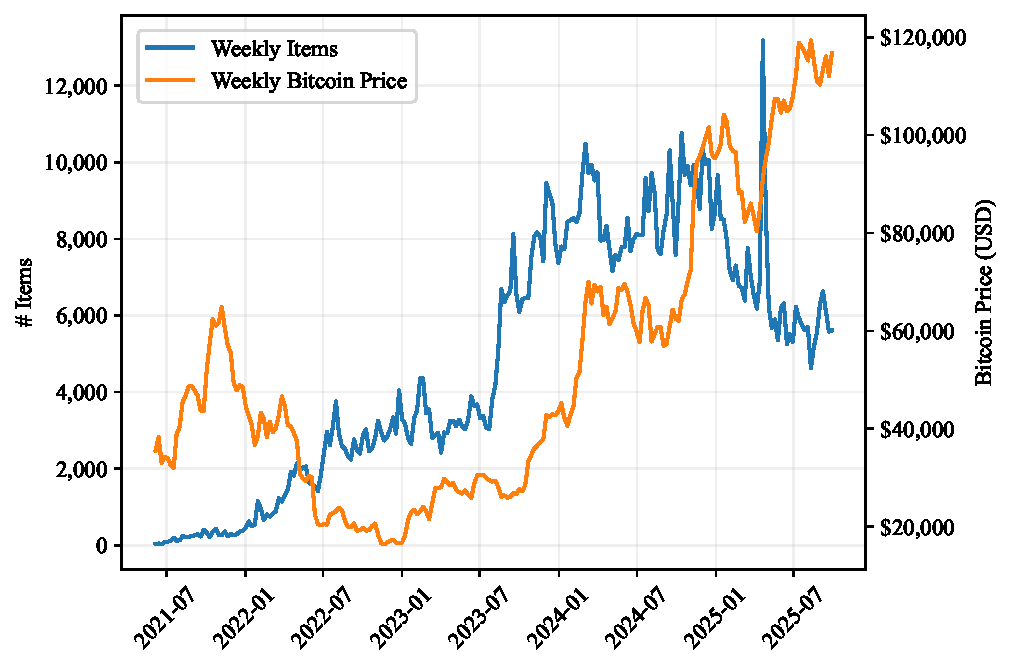
\includegraphics{results/fig_weekly_items.pdf}
\end{adjustbox}
\end{center}
\footnotesize \textit{Note:} Shows the number of items posted on Stacker News by week along with the weekly Bitcoin price. Weekly Bitcoin price is calculated as the average of the midpoint between daily highs and lows as reported by CoinMarketCap.com. 
\end{figure}

\pagebreak

\begin{figure}[H]
\caption{Posting Cost Histories for Select Territories} \label{fig_posting_fee_histories}
\vspace{-0.6cm}
\begin{center}
\begin{adjustbox}{width=\textwidth}
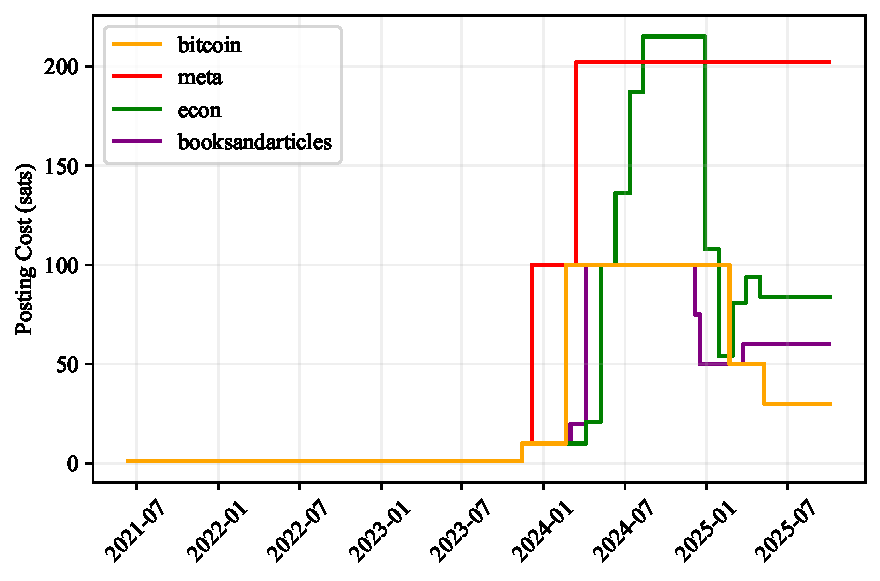
\includegraphics{results/fig_territory_posting_fees.pdf}
\end{adjustbox}
\end{center}  
\footnotesize \textit{Note:} This figure shows the territory fee path for four selected territories. The territories were selected both for their popularity and to highlight the differences in timing and magnitude of fee changes across territories. 
\end{figure}

\pagebreak

\begin{figure}[H]
\caption{Post Quality Event Study}
\label{fig_post_quality_event_study}
\vspace{-0.6cm}
\begin{center}
\begin{adjustbox}{width=\textwidth}
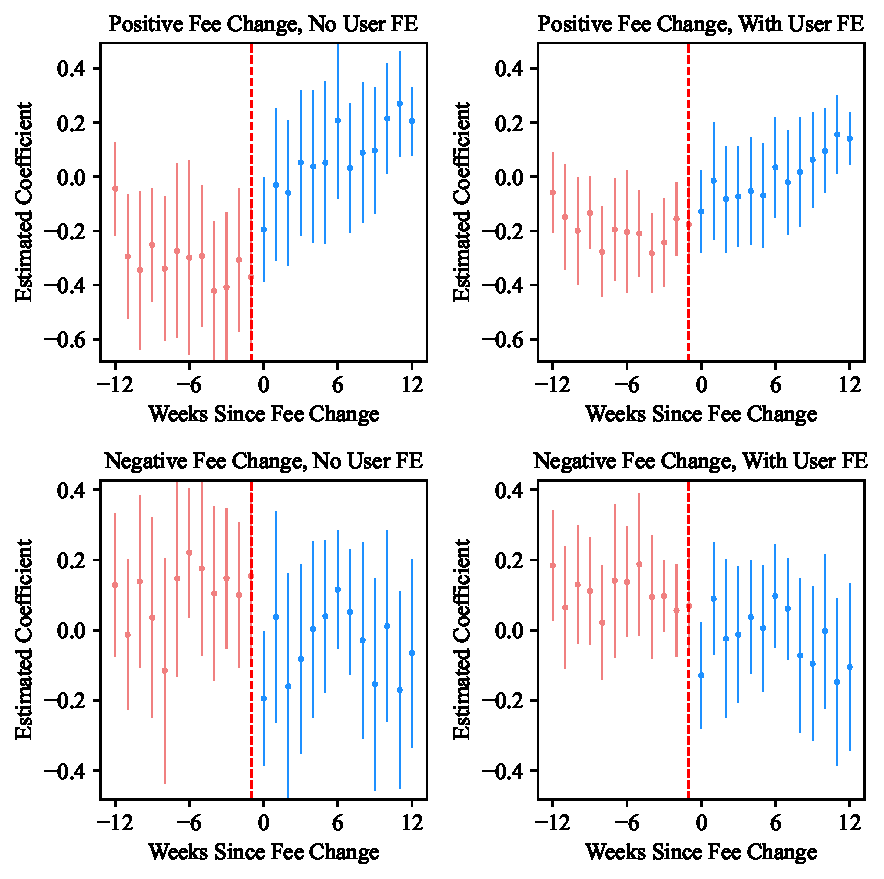
\includegraphics{results/fig_post_quality_event_study.pdf}
\end{adjustbox}
\end{center}
\footnotesize \textit{Note:} Shows estimated coefficients and 95\% confidence intervals from the post quality event study regression specified by equation \eqref{eq_post_quality_event_study}. All regressions shown include territory-operator fixed effects and week fixed effects. 
\end{figure}

\pagebreak

\begin{figure}[H]
\caption{Post Quantity Event Study}
\label{fig_post_quantity_event_study}
\vspace{-0.6cm}
\begin{center}
\begin{adjustbox}{width=\textwidth}
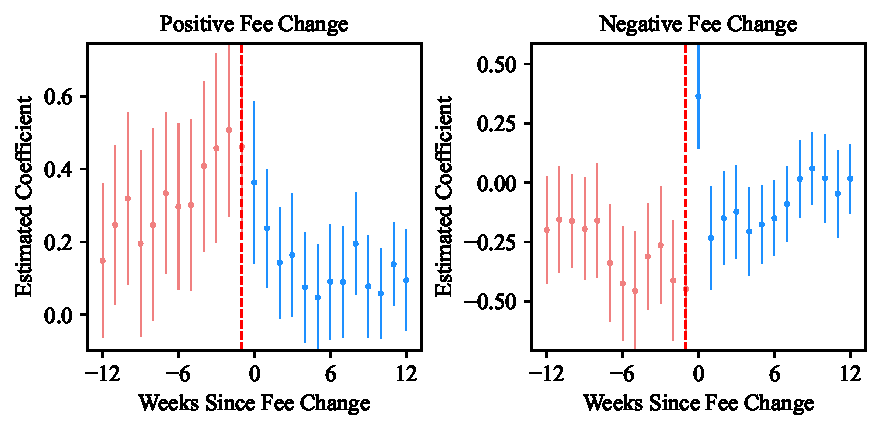
\includegraphics{results/fig_post_quantity_event_study.pdf}
\end{adjustbox}
\end{center}
\footnotesize \textit{Note:} Shows estimated coefficients and 95\% confidence intervals from the post quantity event study regression specified by equation \eqref{eq_post_quantity_event_study}. All regressions shown include territory fixed effects and week fixed effects. 
\end{figure}

\pagebreak

\begin{figure}[H]
\caption{Post Quality Over Time} \label{fig_v4v_q_trend}
\vspace{-0.8cm}
\begin{center}
\begin{adjustbox}{width=\textwidth}
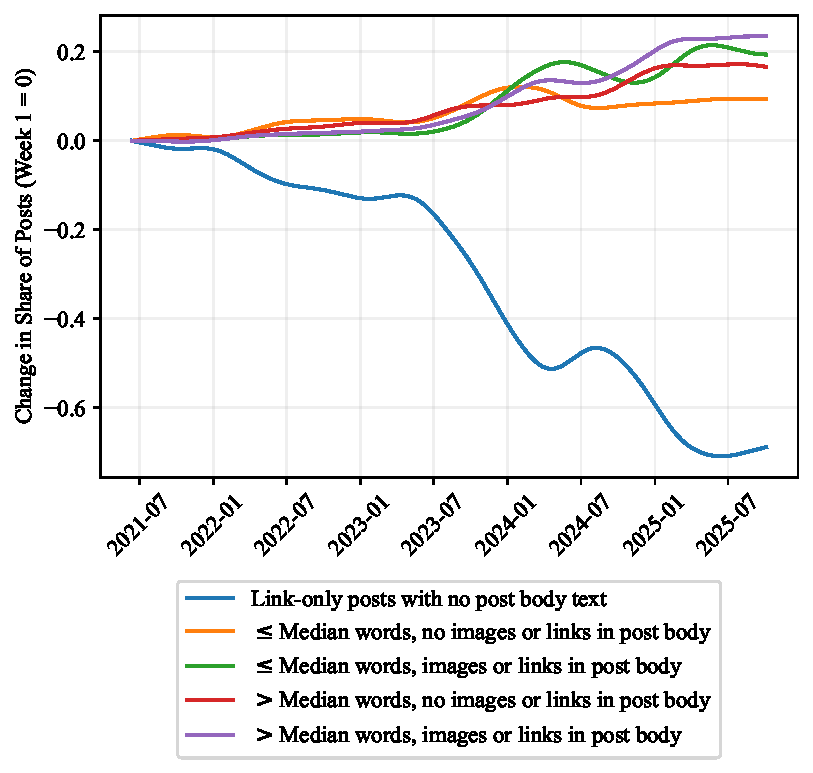
\includegraphics{results/fig_v4v_q_trend.pdf}
\end{adjustbox}
\end{center}
\vspace{-0.5cm}
\footnotesize \textit{Note:} Shows the average post quality as measured by objective post attributes ($q_{ij}$) for each week. See Section \ref{sec_v4v} for details. 
\end{figure}


\pagebreak
\begin{table}[H]
\centering
\caption{Effect of Posting Cost on Post Quality} 
\vspace{0.2cm}
\label{tbl_sats48_cost_reg}
\begin{threeparttable}
\begin{tabular}{lcccc} 
\toprule
 & \multicolumn{4}{c}{\textit{Dependent variable:}} \\ 
\cline{2-5} 
 & \multicolumn{4}{c}{log(Zaps)} \\ 
 & (1) & (2) & (3) & (4)\\ 
\midrule
 &  &  &  &  \\
log(Posting Cost)  & 0.393$^{***}$ & 0.273$^{***}$ & 0.219$^{***}$ & 0.091$^{**}$ \\
 & (0.048) & (0.058) & (0.050) & (0.044) \\
Constant  & 2.530$^{***}$ &  &  &  \\
 & (0.076) &  &  &  \\
 & & & & \\
Territory FE            & N & Y & Y & Y \\
Week FE                 & N & Y & Y & Y \\
Territory Operator FE   & N & N & Y & Y \\
User FE                 & N & N & N & Y \\
& & & & \\
Observations  & 179,480 & 179,477 & 179,476 & 178,197 \\ [1.8ex]
\bottomrule
\end{tabular} 
\begin{tablenotes}[flushleft]
\footnotesize
\item Robust standard errors in parentheses. * $p<0.1$, ** $p<0.05$, *** $p<0.01$.
\item \textit{Notes:} Regression of number of sats a post earns in the first 48 hours on posting cost. The unit of observation is a post. Standard errors are clustered by territory.
\end{tablenotes}
\end{threeparttable}
\end{table}
 
\pagebreak
\begin{table}[H]
\centering
\caption{Effect of Posting Cost on Post Quantity} \label{tbl_posts_cost_reg}
\begin{threeparttable}
\begin{tabular}{@{\extracolsep{5pt}}lccc} 
\\[-1.8ex]\hline 
\hline \\[-1.8ex] 
 & \multicolumn{3}{c}{\textit{Dependent variable:}} \\ 
\cline{2-4} 
\\[-1.8ex] & \multicolumn{3}{c}{log(Posts)} \\ 
\\[-1.8ex] & (1) & (2) & (3)\\ 
\hline \\[-1.8ex] 
log(Posting Cost)  & -0.242$^{***}$ & -0.266$^{***}$ & -0.265$^{***}$ \\
 & (0.079) & (0.063) & (0.074) \\
Constant  & 3.328$^{***}$ &  &  \\
 & (0.415) &  &  \\
& & & \\
\hline \\ [-1.8ex]
Territory FE            & N & Y & Y \\
Week FE                 & N & Y & Y \\
Territory Operator FE   & N & N & Y \\
Observations  & 6,023 & 6,020 & 6,020 \\ \hline \hline
\end{tabular} 
\begin{tablenotes}[flushleft]\footnotesize
\item[] \parbox[t]{\linewidth}{%
\hfill * $p<0.1$, ** $p<0.05$, *** $p<0.01$.
}
\item \textit{Notes:} Regression of number of posts in a territory on posting costs for that week. The unit of observation is a territory-week. Standard errors are clustered by territory.
\end{tablenotes}
\end{threeparttable}
\end{table}
 
\pagebreak
\begin{table}[H]
\centering
\caption{Post Types Summary}
\vspace{0.2cm}
\label{tbl_post_types_summary}
\begin{adjustbox}{max width=\textwidth}
\begin{threeparttable}
\begin{tabular}{lrrr}
\toprule
& \makecell{Number\\of posts} & \makecell{Avg. sats\\received in\\first 48 hours} & \makecell{Avg. replies\\received in\\first 48 hours} \\ \midrule
& & & \\
Link-only posts with no post body text & 90,154 & 167 & 1.3 \\ [1ex]
$\leq$Median words, no images or links in post body & 19,385 & 296 & 5.1 \\ [1ex]
$\leq$Median words, images or links in post body & 23,517 & 271 & 3.1 \\ [1ex]
$>$Median words, no images or links in post body & 19,172 & 564 & 6.8 \\ [1ex]
$>$Median words, images or links in post body & 23,629 & 1,112 & 6.9 \\ [1ex]

& & & \\
\bottomrule
\end{tabular}
\begin{tablenotes}
\item {\textit{Notes: } This table reports the number of posts and the average amount of sats and replies received in the first 48 hours, for each post type.}
\end{tablenotes}
\end{threeparttable}
\end{adjustbox}
\end{table}

\pagebreak
\begin{table}[H]
\centering
\caption{Effect of Observed Tip Feedback on Post Type Choice}
\vspace{0.2cm}
\label{tbl_learning}
\begin{adjustbox}{max width=\textwidth}
\begin{threeparttable}
\begin{tabular}{lcccccc}
\toprule
 & \multicolumn{6}{c}{Observed feedback weighted by:} \\
 & \multicolumn{2}{c}{Uniform} & \multicolumn{2}{c}{Recency} & \multicolumn{2}{c}{\makecell{Distance to user's\\peak activity}} \\ [1ex]
 & (1) & (2) & (3) & (4) & (5) & (6) \\
\midrule
 &  &  &  &  &  &  \\
Observed Tips  & 1.191$^{**}$ & 1.328$^{***}$ & 1.311$^{***}$ & 1.304$^{***}$ & 1.244$^{***}$ & 1.371$^{***}$ \\
 & (0.487) & (0.505) & (0.433) & (0.443) & (0.466) & (0.482) \\ [1.8ex]
Observed Tips $\times$ User's Experience  & -0.259$^{***}$ & -0.252$^{***}$ & -0.266$^{***}$ & -0.266$^{***}$ & -0.249$^{***}$ & -0.246$^{***}$ \\
 & (0.091) & (0.083) & (0.086) & (0.086) & (0.088) & (0.082) \\ [1.8ex]
User Excess Tips  &  & 0.221$^{**}$ &  & -0.011$^{}$ &  & 0.177$^{**}$ \\
 &  & (0.091) &  & (0.048) &  & (0.083) \\ [1.8ex]
 &  &  &  &  &  &  \\
Type-Specific Intercepts & Y  & Y  & Y  & Y  & Y  & Y  \\
Type-Specific Linear Time Trends & Y  & Y  & Y  & Y  & Y  & Y  \\
 &  &  &  &  &  &  \\
Observations  & 82,173 & 82,173 & 82,173 & 82,173 & 82,173 & 82,173 \\ 
McFadden's Pseudo-R$^2$ & 0.072 & 0.079 & 0.075 & 0.075 & 0.071 & 0.077 \\ [1.8ex]
\bottomrule
\end{tabular}
\begin{tablenotes}[flushleft]
\footnotesize
\item[] \parbox[t]{\linewidth}{%
\hfill * $p<0.1$, ** $p<0.05$, *** $p<0.01$.
}
\item \textit{Notes:} This table reports estimated coefficients for the conditional logit model of post type choice described in Section \ref{sec_v4v_model}. Each unit of observation is a user $i$'s choice to make a post of type $c$ at time $t$. The user chooses the post type based on their observation of tips earned by posts of each type. ``Observed Tips'' is a weighted average of ln(sats) earned on posts of each type $c$ prior to time $t$. See Section \ref{sec_v4v} for a description of the model and weighting functions. ``User's Experience'' is the $\ln$ of the number of posts the user $i$ has made up to time $t$. ``User Excess Tips'' is the weighted average of the user's own ln(sats) for each post type $c$ earned in excess of the overall weighted average for that post type. Standard errors are clustered by user.
\end{tablenotes}
\end{threeparttable}
\end{adjustbox}
\end{table}

\pagebreak
\begin{table}[H]
\centering
\caption{Effect of Profitability on User Exit} 
\vspace{0.2cm}
\label{tbl_profitability_analysis}
\begin{adjustbox}{max width=\textwidth}
\begin{threeparttable}
\begin{tabular}{lcccc} 
\toprule
 & \multicolumn{4}{c}{\textit{Dependent variable:}} \\ 
 & \multicolumn{4}{c}{Whether user becomes inactive} \\ [1ex]
 & (1) & (2) & (3) & (4) \\ 
\midrule
 &  &  &  &  \\
Unprofitable in last 8 weeks  & 0.105$^{***}$ & 0.062$^{***}$ & 0.060$^{***}$ & 0.055$^{***}$ \\
 & (0.003) & (0.003) & (0.003) & (0.003) \\ [1ex] 
$\ldots \times$ BTC price appreciation in last 8 weeks  &  &  &  & 0.056$^{***}$ \\
 &  &  &  & (0.014) \\ [1ex] 
log(Items posted in last 8 weeks)  &  & -0.029$^{***}$ & -0.029$^{***}$ & -0.029$^{***}$ \\
 &  & (0.001) & (0.001) & (0.001) \\ [1ex] 
Constant  & 0.079$^{***}$ & 0.157$^{***}$ &  &  \\
 & (0.001) & (0.002) &  &  \\ [1ex] 
& & & & \\
Week FE & N & N & Y & Y \\
 & & & & \\
Observations  & 92,956 & 92,956 & 92,956 & 92,956 \\ 
R$^2$  & 0.018 & 0.042 & 0.048 & 0.048 \\ [1.8ex] 
\bottomrule
\end{tabular} 
\begin{tablenotes}[flushleft]\footnotesize
\item[] \parbox[t]{\linewidth}{%
\hfill * $p<0.1$, ** $p<0.05$, *** $p<0.01$.
}
\item \textit{Notes:} Linear probability model of whether a user becomes inactive in a given week. A user becomes inactive if they start a four or more week consecutive period of no activity. The unit of observation is a user-week.
\end{tablenotes}
\end{threeparttable}
\end{adjustbox}
\end{table}


\pagebreak

\appendix

\section*{Online Appendix}

\section{A Model}

First, we develop a simple model of posting behavior to ground our empirical work. Then, we test whether the predictions of the model are supported by the data.

\subsection{A model of pay-to-post}

We envision a model in which a user receives ``post ideas'' as a Poisson arrival process with rate $\gamma$. Post ideas arrive with a quality level $q$, which affects how other users respond to the post, and an intrinsic motivation to post it, $\epsilon$. The level of internal motivation may be correlated with post quality, and they are drawn from a joint probability density function $f(q,\epsilon)$. We allow different users to draw from different distributions of $(q,\epsilon)$, but for now we focus on the decisions of a single user.

By Bayes' Rule, $f(q, \epsilon) = f_{\epsilon|q} (\epsilon | q) f_q (q)$, where $f_{\epsilon|q}(\cdot)$ is the conditional density of $\epsilon$ given $q$, and $f_q(\cdot)$ is the marginal density of $q$. We assume that $f_{\epsilon|q}(\cdot)$ is strictly log-concave and weakly satisfies the monotone likelihood ratio property in $\epsilon$ with respect to $q$:

\begin{assumption}[Log Concavity]\label{asm_logconcavity}
For each $q$, $f_{\epsilon|q}(\cdot | q)$ is strictly log-concave; that is, $\ln f_{\epsilon|q} (\epsilon | q)$ is strictly concave in $\epsilon$.
\end{assumption}
\begin{assumption}[Monotone Likelihood Ratio Property]\label{asm_mlrp}
For any $q_2 > q_1$, the likelihood ratio of the conditional densities,
\begin{align*}
\ell(\epsilon;q_1, q_2) = \frac{f_{\epsilon|q}(\epsilon|q_2)}{f_{\epsilon|q}(\epsilon|q_1)}
\end{align*}
is weakly increasing in $\epsilon$.
\end{assumption}
\noindent \emph{Remark.}  Assumption \ref{asm_logconcavity} limits the heaviness of the tail of the motivation distribution. Intuitively, it ensures that the extreme tail of the motivation distribution is not thick enough to swamp quality selection effects at very high posting costs. It is not a strong assumption, and it is satisfied by most commonly used distributional families, including the normal and logistic distributions.\footnote{Weaker, local conditions about the hazard rate in the neighborhood of the current posting cost would also suffice, but we state the stronger condition of global log-concavity for simplicity. Moreover, strict log-concavity is assumed for simplicity, but it suffices to assume either strict log-concavity or strict monotone likelihood ratio property; we do not need strictness for both.}

Assumption \ref{asm_mlrp} is a non-negative dependence condition between post quality $q$ and intrinsic motivation $\epsilon$. Informally, it says that higher quality ideas tend to come with (weakly) higher intrinsic desire to post: when $q$ is higher, the distribution of $\epsilon$ shifts to the right. Independence between $\epsilon$ and $q$ is allowed as a special case, but the assumption rules out systematic negative dependence. In our context, this means that users who receive a high quality post idea are also (weakly) more likely to feel a strong intrinsic desire to post it. As we shall document later, this is consistent with users' self reported perceptions of their own motivations. \hfill \qedsymbol

~

\noindent Once a post is made, zaps arrive according to a Poisson process. Both the arrival rate of zaps and the amount of each zap are dependent on the quality of the post, $q$. Let $\lambda(q)$ be the arrival rate as a function of $q$, and let $E[z|q]$ be the expected zap amount per zap conditional on $q$. 

Supposing the user has a discount factor of $\rho$, the expected present value of the Poisson stream of zaps is equal to:\footnote{This follows from $V(q) = \int_{0}^{\infty} e^{-\rho t} \lambda(q) E[z|q] dt$.}
\begin{align}
V(q) = \frac{\lambda(q)}{\rho} E \left[z | q\right] \label{eq_V}
\end{align}
We assume that $V(q)$ is continuous and strictly increasing in $q$, which merely says that the expected present value of zaps is higher for higher quality posts:

\begin{assumption}[Monotone Returns to Quality]\label{asm_monotonicity}
$V(q) = \frac{\lambda(q)}{\rho} E[z|q]$ is continuous and strictly increasing in $q$.
\end{assumption}

~

\noindent  The user will make the post if their expected present value of zaps plus their intrinsic motivation is greater than the posting cost $c$:
\begin{align}
\text{Post} = 1 \text{ if } V(q) + \epsilon > c \text{ and } 0 \text{ otherwise }
\end{align}
From the perspective of the user, $c$ is fixed and known at the time of the post.

We now demonstrate conditions under which an increase in posting cost $c$ will lead to fewer posts, but higher quality posts.

\begin{proposition} \label{prop_pay_to_post}
Suppose Assumptions \ref{asm_logconcavity}-\ref{asm_monotonicity} hold. Then an increase in $c$:
\begin{enumerate}[label=(\roman*)]
\item strictly decreases the probability that the post idea is posted, and
\item strictly increases the expected quality of posts, conditional on posting.
\end{enumerate}
\end{proposition}

\begin{proof}
A proof is provided in the appendix.
\end{proof}

\noindent \emph{Remark.} Proposition \ref{prop_pay_to_post} implies that when posting cost increases, users are less likely to post, but that when they do post, the average quality of the post is higher. Although the proposition is stated from the perspective of a single user, we note that as long as the global joint distribution of $(q,\epsilon)$ holds to Assumptions \ref{asm_logconcavity} and \ref{asm_mlrp}, and if Assumption \ref{asm_monotonicity} also holds for all users, then Proposition \ref{prop_pay_to_post} applies in the aggregate, even if users have heterogeneous marginal densities for $q$ and $\epsilon$. 

The result of Proposition \ref{prop_pay_to_post} extends to a setting with multiple territories. Users post in the territory $j$ that maximizes $V_j(q_j) + \epsilon_j - c_j$, provided it is positive. When territory $j$ raises its posting cost $c_j$, users' outside options are unaffected, so the same logic applies: as long as the population-level joint distribution of quality and motivation within each territory satisfies Assumptions \ref{asm_logconcavity}-\ref{asm_monotonicity}, a territory that raises its posting cost will see fewer but higher quality posts. \hfill \qedsymbol




\subsubsection*{Proof of Proposition \ref{prop_pay_to_post}}

\begin{proof}
A post idea $(q, \epsilon)$ is posted if and only if $\epsilon > c - V(q)$. Define $\pi(q,c)$ as the probability (over $\epsilon$) that a post of quality is posted when the cost is $c$:
\begin{align*}
\pi(q,c) &= P(\epsilon > c - V(q)) 
\end{align*}
$\pi(q,c)$ is equivalent to the survival function of $\epsilon|q$, evaluated at $c - V(q)$: $\pi(q,c) = S_{\epsilon|q}(c - V(q) | q)$.
\begin{enumerate}[label=(\roman*)]
\item The unconditional probability of posting is:
\begin{align*}
P(\text{post}) = \int S_{\epsilon|q}(c-V(q)|q)f_q(q)dq
\end{align*}
Since $S_{\epsilon|q}(\cdot|q)$ is a survival function, its first derivative is negative everywhere. An increase in $c$ will therefore reduce the value of $S_{\epsilon|q}(c - V(q))$ at every $q$. Since that is what we are integrating over to get $P(\text{post})$, this strictly reduces $P(\text{post})$. The expected number of posts per unit time is $\gamma P(\text{post})$, so an increase in $c$ strictly reduces the expected number of posts.

\item Take any $c^\prime > c$. The set of ideas that were posted at cost $c$ can be partitioned into two groups:
\begin{itemize}
\item \textbf{Surviving posts.} Ideas that are still posted at cost $c^\prime$, i.e. $V(q) + \epsilon > c^\prime$
\item \textbf{Marginal posts.} Ideas that are posted at $c$ but not at $c^\prime$, i.e. $c < V(q) + \epsilon < c^\prime$.
\end{itemize}
By the Law of Iterated Expectations,
\begin{align*}
E[q | \text{post at } c] = \alpha E[q | \text{surviving}] + (1-\alpha) E[q | \text{marginal}]
\end{align*}
where $\alpha = P(\text{surviving} | \text{post at } c)$. Noting that $E[q|\text{post at } c^\prime] = E[q|\text{surviving}]$, we rearrange the above equation to obtain:
\begin{align*}
E[q|\text{post at } c^\prime] - E[q|\text{post at } c] = (1-\alpha) \left( E[q|\text{surviving}] - E[q|\text{marginal}\right)
\end{align*}
Thus, to show that expected post quality is increasing in $c$, it suffices to show that the expected quality of the surviving posts is always higher than the expected quality of the marginal posts. 

To demonstrate this, it is sufficient to establish that for any $q_2 > q_1$, the ratio $\pi(q_2,c)/\pi(q_1,c)$ is strictly increasing in $c$. Intuitively, this says that as costs rise, higher quality posts retain a larger share of the posting probability relative to lower quality ideas. This would imply that the marginal posts are tilted towards lower quality than surviving posts.

We write:
\begin{align*}
\frac{\pi(q_2,c)}{\pi(q_1,c)} = \frac{S_{\epsilon|q}(c-V(q_2)|q_2)}{S_{\epsilon|q}(c-V(q_1)|q_1)} \label{eq_prob_ratio}
\end{align*}
Define the hazard rate: $h(\epsilon|q) = f_{\epsilon|q}(\epsilon|q) / S_{\epsilon|q}(\epsilon|q)$. Differentiating $\pi(q_2,c)/\pi(q_1,c)$ with respect to $c$ shows us that the ratio is increasing in $c$ if and only if:
\begin{align*}
h(c - V(q_1) | q_1) > h(c - V(q_2) | q_2)
\end{align*}
The proof now proceeds in two parts. 

\paragraph{Claim 1.} First, we show that $h(\epsilon | q_1) \geq h(\epsilon | q_2)$ for any $q_2 > q_1$. By the MLRP, for any $t > \epsilon$, we have that $\ell(t; q_1, q_2) \geq \ell(\epsilon; q_1, q_2)$, which rearranges to:
\begin{align*}
f_{\epsilon|q}(t|q_2) f_{\epsilon|q}(\epsilon|q_1) \geq f_{\epsilon|q}(\epsilon|q_2) f_{\epsilon|q}(t|q_1)
\end{align*}
Integrating both sides over $t$ from $\epsilon$ to $\infty$ gives us:
\begin{align*}
S_{\epsilon|q}(\epsilon|q_2) f_{\epsilon|q}(\epsilon|q_1) \geq S_{\epsilon|q}(\epsilon|q_1) f_{\epsilon|q}(\epsilon|q_2)
\end{align*}
which rearranges to $h(\epsilon|q_1) \geq h(\epsilon | q_2)$ as was to be demonstrated.

\paragraph{Claim 2.} Now, we show that $h(\epsilon|q)$ is increasing in $\epsilon$ for each $q$. Take the derivative of $h(\epsilon|q)$ with respect to $\epsilon$. The sign is equal to the sign of:
\begin{align*}
f_{\epsilon|q}(\epsilon|q)^2 + f^\prime_{\epsilon|q}(\epsilon|q) S_{\epsilon|q}(\epsilon|q)
\end{align*}
When $f^\prime_{\epsilon|q}(\epsilon|q) \geq 0$, this is immediately positive. When $f_{\epsilon|q}^\prime(\epsilon|q)<0$, we rely on the log-concavity property. Since $f_{\epsilon|q}(\cdot)$ is log-concave, the following holds for every $t > \epsilon$:
\begin{align*}
\ln f_{\epsilon|q} (t|q) < \ln f_{\epsilon|q}(\epsilon|q) + (t-\epsilon) \frac{f_{\epsilon|q}^\prime(\epsilon|q)}{f_{\epsilon|q}(\epsilon|q)}
\end{align*}
Exponentiating both sides:
\begin{align*}
f_{\epsilon|q} (t|q) < f_{\epsilon|q}(\epsilon|q) \exp\left[ (t-\epsilon) \frac{f_{\epsilon|q}^\prime(\epsilon|q)}{f_{\epsilon|q}(\epsilon|q)} \right]
\end{align*}
Now integrating over $t$ from $\epsilon$ to $\infty$:
\begin{align*}
S_{\epsilon|q} (\epsilon | q) &< f_{\epsilon|q}(\epsilon|q) \int_{\epsilon}^\infty \exp\left[ (t-\epsilon) \frac{f_{\epsilon|q}^\prime(\epsilon|q)}{f_{\epsilon|q}(\epsilon|q)} \right] dt \\
& = - \frac{f_{\epsilon|q}(\epsilon|q)^2}{f^\prime_{\epsilon|q}(\epsilon|q)}
\end{align*}
Since $f^\prime_{\epsilon|q}(\epsilon|q) < 0$, this can be rearranged to:
\begin{align*}
f_{\epsilon|q}(\epsilon|q)^2 + f^\prime_{\epsilon|q}(\epsilon|q) S_{\epsilon|q}(\epsilon|q) > 0
\end{align*}
which was to be demonstrated. Thus, $h(\epsilon|q)$ is strictly increasing in $\epsilon$ for all $q$.

By the monotonicity assumption, $c - V(q_1) > c - V(q_2)$. By Claim 2, this implies that $h(c - V(q_1)|q_1) > h(c-V(q_2)|q_1)$. By Claim 1, $h(c-V(q_2) | q_1) \geq h(c-V(q_2) | q_2)$. Together, we have $h(c - V(q_1)|q_1) > h(c-V(q_2)|q_2)$, which was to be demonstrated. 
\end{enumerate}
\end{proof}


\subsubsection*{Proof of Proposition \ref{prop_v4v}}

\begin{proof}
Given $\hat{\theta}$, the user's expected utility from effort is:
\begin{align*}
U(e;\hat{\theta}) = E_{q,\epsilon|e} \left[ \max \left\{ \exp (\hat{\theta} + q) - c + \epsilon, 0 \right\} \right] - \kappa(e)
\end{align*}
It suffices to show that $U(e; \hat{\theta})$ is supermodular in $(e, \hat{\theta})$. For any $\hat{\theta}_2 > \hat{\theta}_1$:
\begin{align*}
U(e;&\hat{\theta}_2) - U(e;\hat{\theta}_1) = \\
& E_{q,\epsilon|e}\left[ \max \left\{ \exp( \hat{\theta}_2 + q) - c + \epsilon, 0\right\} - \max \left\{ \exp( \hat{\theta}_1 + q) - c + \epsilon, 0 \right\} \right]
\end{align*}
The integrand is supermodular in $(\hat{\theta},q)$ because  $\exp(\hat{\theta} + q)$ is supermodular in $(\hat{\theta}, q)$ and because the $\max$ operator is convex and increasing. Furthermore, since $F(q|\epsilon;e)$ satisfies FOSD in $e$, it follows immediately $U(e;\hat{\theta}_2)-U(e;\hat{\theta}_1)$ is increasing in $e$, and hence $U(e;\hat{\theta})$ is supermodular in $(e,\hat{\theta}).$
\end{proof}

\section{Methodological Detail - Text Embeddings}

Text embeddings were computed for each post by inputting the post text into \mbox{OpenAI's} \texttt{text-embedding-3-small} embedding model. The embedding model computes a 1,536 dimensional embedding vector for each post that encodes the meaning of the text in such a way that two posts with similar text will have a small distance between their embedding vectors. The raw embedding dimensions are learned from a large general purpose training corpus and are not tailored to the structure of our dataset. We therefore compute the principal components of the raw embedding vectors using our corpus. The principal components are orthogonal linear combinations of the original 1,536 embedding dimensions that explain the greatest variation across posts in our data. Figure \ref{fig_text_scree_plot} shows the scree plot of the principal components analysis, for the first \gn{NumPCAComponentsShow} components. To keep our regression in \eqref{eq_zreg} parsimonious, we decided to use only the first \gn{TextPCAK} components in the analysis. These components explain  \gn{TextPCAPctExplained}\% of the total variation,  but our results in Section \ref{sec_v4v} are robust to the specific choice of how many components to use. After running regression \eqref{eq_zreg}, we inspected the embedding dimensions that were most predictive of zaps. The first most predictive dimension appears to capture meta-posts (not necessarily in the \texttt{meta} territory) about Stacker News itself, such as tips for how to post and earn more sats. The second most predictive dimension appears to capture posts about geopolitical and macroeconomic events, such as a personal discussion about elections in Venezuela. The third dimension most predictive dimension appears to capture posts that ask questions about personal finance. We note that, although these embedding dimensions are the most strongly associated with zaps, other predictive aspects of the text content may not align with any single dimension and may instead be captured by combinations of dimensions. We therefore treat the embedding components primarily as control variables in the regression and avoid over-interpreting individual coefficients or assigning strong substantive meaning to any single dimension.

\pagebreak

\begin{figure}[H]
\caption{Scree Plot for Post Text Embeddings}
\label{fig_text_scree_plot}
\vspace{-0.6cm}
\begin{center}
\begin{adjustbox}{width=\textwidth}
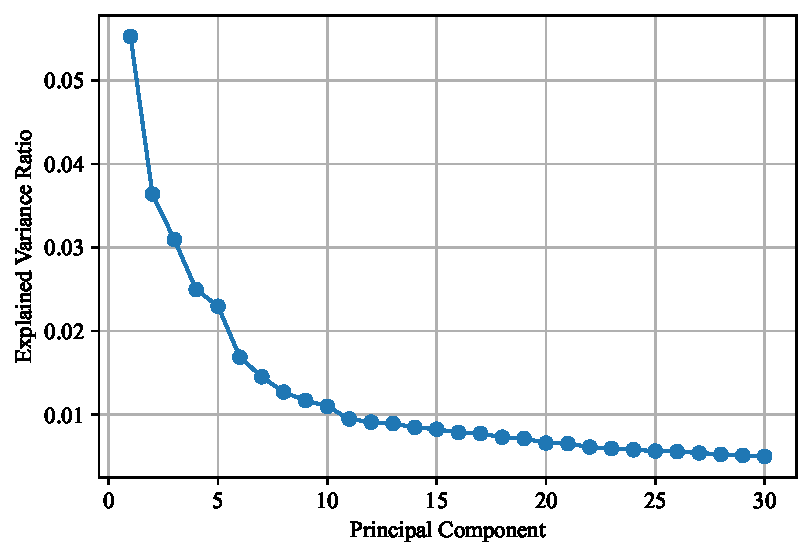
\includegraphics{results/fig_text_scree_plot.pdf}
\end{adjustbox}
\end{center}
\footnotesize \textit{Note:} Shows the scree plot for post text embeddings, indicating the explained variance ratio for each principal component. 
The total explained variance at $K=10$ is \gn{TextPCAPctExplained}\%.
\end{figure}



\end{document}

